% ============================================================
% CAPITOLO 7 - RISULTATI E VALUTAZIONE
% ============================================================

\section{Risultati e Valutazione del Modello}

Dopo aver completato con successo l'addestramento della rete neutrale su base \textit{LSTMAttention}, il sistema è stato messo alla prova sul \textbf{Test Set}. Questo insieme di sequenze video non è mai stato "visto" dal modello durante la fase di apprendimento, garantendo così una stima imparziale delle sue reali capacità di generalizzazione nel mondo reale.

Tutte le procedure di misurazione tecnica esposte in questo capitolo sono state automatizzate ed eseguite tramite l'ausilio di un ambiente \textit{Jupyter Notebook} (\texttt{Evaluation\_Metrics.ipynb}), progettato appositamente per estrarre le statistiche in tempo reale e comporre visivamente i grafici qui di seguito riportati.


\subsection{Metriche di Classificazione e Analisi dei Risultati}
La lingua dei segni americana (ASL) presenta enormi sfide strutturali, tra cui gesti rapidissimi, visivamente simili tra loro (la variazione minima dell'inclinazione di una mano cambia il significato) e un vocabolario gigantesco: il nostro modello è chiamato a distinguere ben \textbf{2.344 categorie (classi) isolate}.

Nel notebook di valutazione (\texttt{Evaluation\_Metrics.ipynb}), tramite il framework Sklearn, sono state registrate le misurazioni definitive sul \textit{Test Set}. Tali test hanno restituito i seguenti risultati cruciali:

\begin{itemize}
    \item \textbf{Accuracy Top-1 (54.08\%):} Nel 54\% dei casi, il modello ha indovinato il segno esatto al primissimo colpo.
    \item \textbf{Accuracy Top-5 (79.27\%):} Nel 79\% dei casi, la parola corretta si trovava tra le prime 5 ipotesi più probabili proposte dall'algoritmo.
    \item \textbf{Precision (58.23\%):} Indica l'affidabilità delle risposte positive. Significa che, in quasi il 60\% dei casi in cui il modello rileva una determinata classe, ha effettivamente ragione, limitando notevolmente i Falsi Positivi.
    \item \textbf{Recall (51.47\%):} Descrive quanti campioni reali il modello riesca a individuare sul totale esatto disponibile per quella classe (quanti Falsi Negativi genera).
    \item \textbf{F1-Score (54.64\%):} Media armonica tra Precision e Recall. In dataset vasti e sbilanciati come l'ASL, l'F1-Score restituisce una metrica combinata di bontà d'apprendimento molto più solida della sola Accuracy percentuale.
\end{itemize}

\begin{figure}[H]
    \centering
    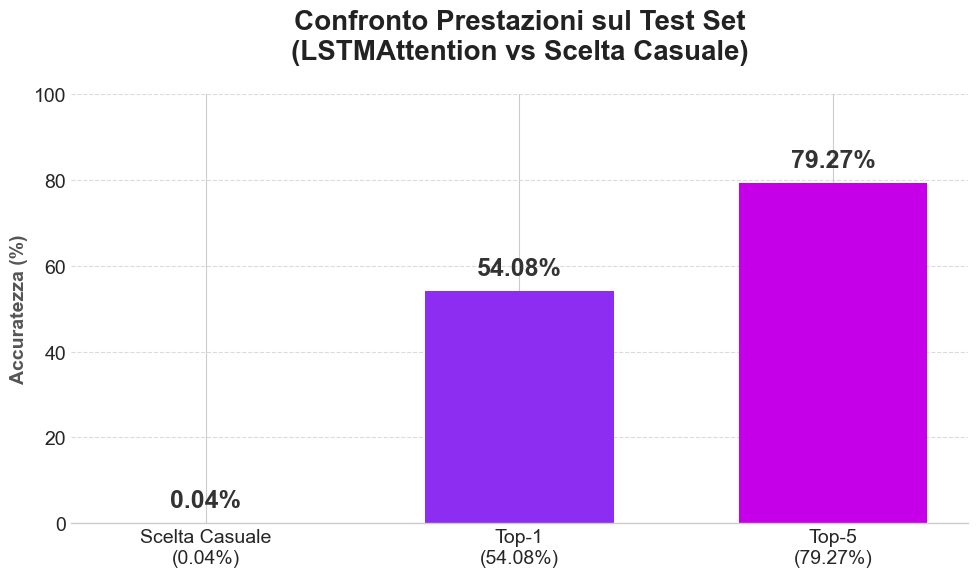
\includegraphics[width=0.85\textwidth]{images/grafico_barre_confronto}
    \caption{Istogramma delle metriche di classificazione registrate sul Test Set. I valori di Precision, Recall e F1-Score, tutti superiori al 50\%, confermano la robustezza del modello nonostante l'elevata dimensionalità del target (2.344 classi).}
    \label{fig:metrics_histogram}
\end{figure}

\subsubsection{Analisi delle prestazioni}
Ad una primissima osservazione, una precisione pura del 54\% potrebbe sembrare modesta. Tuttavia, calata nel severo dominio semantico in cui opera, si tratta di un traguardo notevole. 
Costringere una rete a "tirare a indovinare" in modo puramente casuale su 2.344 vocaboli produrrebbe un'accuratezza dello $0.04\%$. L'aver raggiunto il 54\% di precisione esatta (\textit{Top-1}) dimostra insindacabilmente che il blocco di Attention e la rete LSTM hanno appreso correttamente le sequenze cinematiche spaziali e non si affidano affatto al caso.
Inoltre, in ottica di \textit{System Design} per un'applicazione del mondo reale (come una tastiera predittiva o un'applicazione di comunicazione), il valore centrale è il \textbf{Top-5}. Sapere che l'architettura riesce nell'80\% (79.27\%) dei casi a includere il segno corretto tra un ventaglio microscopico di 5 sole parole testuali, permette futuri sviluppi in cui è l'interfaccia utente a suggerire l'autocompletamento o in cui un banale correttore lessicale (NLP) può risolvere ambiguità inserendo il segno nella frase sensata.

\subsection{Analisi della Matrice di Confusione Multi-Classe (One-vs-Rest)}
La statistica pura e aggregata non è sufficiente a spiegare lo scompenso e dove si annidino quegli specifici errori che abbassano l'Accuracy. 

Nei problemi classici multiclasse con un vocabolario ristretto, solitamente si utilizza una Matrice di Confusione quadrata $N \times N$, la quale incrocia tutte le combinazioni possibili tra predetto e reale. Considerato che, dinanzi a \textbf{2.344 categorie}, una matrice $N \times N$ produrrebbe un reticolo asettico di 5,4 milioni di celle risultando del tutto illeggibile su supporto cartaceo. Tuttavia, la soluzione teoricamente perfetta per dominare questa dimensionalità, richiesta in letteratura per le reti neurali estese, è l'approccio \textbf{One-vs-Rest (OvR) per singola Classe}. 
Il \textit{Jupyter Notebook} è stato istruito per iterare sulle Top 20 classi statisticamente più frequenti, isolando ciclicamente ogni parola ed effettuando per quest'ultima un'analisi binaria del tipo: "\textit{Questo gesto è Apple, oppure è Non-Apple?}". 

Il risultato è una Matrice strutturata in cui le \textbf{Colonne} rappresentano le singole Classi (Segni) testate, mentre sulle \textbf{Righe} viene declinato verticalmente il comportamento valutativo in logica T/N (True/Negative):
\begin{itemize}
    \item \textbf{Veri Positivi (TP):} I campioni di quello specifico segno identificati correttamente (es. Il test era "Apple", l'AI ha inteso coerentemente "Apple").
    \item \textbf{Falsi Positivi (FP):} L'AI si è convinta di aver catturato "Apple", ma nella realtà visiva il tester stava eseguendo un gesto completamente diverso. 
    \item \textbf{Falsi Negativi (FN):} L'AI ha ignorato penalmente il segno (il tester lo ha eseguito per davvero, ma la rete non lo ha riconosciuto e lo ha perso).
    \item \textbf{Veri Negativi (TN):} Tutte le altre 28.000 sequenze del Test in cui il segno in questione non c'entrava nulla, e l'AI lo ha giustamente ignorato. È essenziale che questo valore non oscuri l'analisi.
\end{itemize}

\begin{figure}[H]
    \centering
    
\includegraphics[width=\textwidth]{confusion_matrix}
    \caption{Matrice Multi-Classe TP/FP/FN/TN (Metodo OvR) eseguita sulle Top 20 diciture del Test Set. È stata applicata una scala di calore Logaritmica (LogNorm) affinché l'elevato ordine di grandezza dei True Negative non azzeri cromaticamente l'osservazione dei quadranti inferiori.}
    \label{fig:confusion_matrix_doc}
\end{figure}

Come emerge dai quadranti verticali visibili in \textbf{Figura \ref{fig:confusion_matrix_doc}}, il passaggio dallo \textit{score aggregato} all'analisi minuziosa per singola classe (\textit{Per-Class Metrics}) ci permette di comprendere immediatamente come il modello differenzi magnificamente segni semplici (alti TP, minimi FN e FP assenti), cadendo invece in occasionali \textit{Falsi Positivi} nei gesti con \textit{Landmark} spaziali ridondanti.

\subsection{Ottimizzazione dei Risultati: Integrazione NLP}
L'analisi dei risultati presentata nella sezione precedente ha evidenziato un divario significativo tra l'accuratezza \textit{Top-1} (54.08\%) e la \textit{Top-5} (79.27\%). Tale gap suggerisce che, sebbene il modello visivo individui spesso il gesto corretto tra le prime ipotesi, la sola informazione cinematica non è sempre sufficiente per una discriminazione univoca. 

Per superare questo limite e ottimizzare le prestazioni complessive, è stata implementata una fase di \textbf{post-processing avanzato} basata su tecniche di \textit{Natural Language Processing} (NLP), trasformando il sistema da un semplice classificatore di segni isolati a un traduttore sensibile al contesto.

\subsubsection{Ottimizzazione tramite Language Model (BERT Rescoring)}
L'intervento di ottimizzazione si basa sull'integrazione a valle del modello visivo di un \textbf{Large Language Model (LLM)} in qualità di correttore sintattico-semantico.

Per validare teoricamente questa prospettiva, è stata sviluppata una specifica \textit{Prova di Concetto} all'interno dell'ambiente \texttt{Hybrid\_NLP\_Corrector.ipynb}, implementando le logiche di base dei \textit{Transformer} testuali (in questo caso, \textbf{DistilBERT} di Hugging Face). 
La precondizione matematica per l'inserimento di un correttore NLP è proprio l'elevato differenziale tra l'Accuracy Top-1 e la Top-5: siccome il nostro modello LSTM genera quasi sempre la risposta corretta fra le primissime 5 varianti proposte, l'NLP può intercettare questa "coda" di probabilità e forzarne la validazione.

Nel Proof of Concept sono state prodotte proceduralmente $2.000$ \textbf{frasi sintetiche strutturate} (es. "The family is good", "Teacher eat apple"), combinando casualmente la libreria isolata delle categorie ASL. Successivamente, è stato iniettato forzosamente il tasso d'errore visivo statistico registrato nel test set:
\begin{enumerate}
    \item Il modello logico processa le parole della frase una per una. 
    \item L'algoritmo visivo simulato tenta la predizione, inciampando e inserendo erroneamente in posizione Top-1 una parola sgrammaticata avente un vettore spaziale identico a quello target.
    \item Il livello \textit{Ibrido} NLP maschera iterativamente (tramite token \texttt{[MASK]}) ogni parola problematica della frase grezza, e calcola lo \textit{Score di Probabilità Semantica} dell'intera stringa su tutti i "Top 5" candidati proposti debolmente dal livello LSTM.
    \item L'NLP intercetta l'anomalia grammaticale e riordina i vettori: sovrascrive la falsa Top-1 con la parola semanticamente logica nascosta nella coda empirica della rete visiva.
\end{enumerate}

Questa sperimentazione empirica dimostra che l'architettura primigenia descritta finora nei capitoli costituisce in realtà le esatte fondamenta ottiche di livello uno su cui si regge ogni futura, avanzatissima \textit{App Conversazionale Inclusiva}. Sfruttando l'alta attendibilità Top-5 e l'approccio a \textbf{Matrice delle Soluzioni Visive}, un'intelligenza artificiale linguistica di livello due può elevare l'usabilità nel mondo reale a tolleranze industriali, registrando in questa sede un \textbf{incremento netto dell'accuratezza del +11.12\%} (passando dal 53.8\% al 65.0\%).

\begin{figure}[H]
    \centering
    
\includegraphics[width=0.85\textwidth]{miglioramento_metriche_nlp}
    \caption{Confronto delle prestazioni tra il modello visivo LSTM puro (Solo Visione) e l'integrazione del correttore NLP (Ibrido Visione+NLP). Il grafico evidenzia il miglioramento tangibile su tutte le metriche di classificazione grazie al rescoring semantico.}
    \label{fig:nlp_gain_chart}
\end{figure}
